\def\baselinestretch{1}
\chapter{Methodology}

\section{Exploratory data analysis:}
\subsection{Imbalance Data:}


When there is an imbalance within a dataset, it means that there is an uneven distribution of frequencies among different classes. The difference becomes clear when one class has a much larger number of occurrences compared to another. The majority class is the class that occurs more frequently, while the minority class is the class that occurs less frequently. Reduced accuracy is often the outcome of the disparity in class distribution. According to Gosain and Sardana (2017), machine learning algorithms often show improved accuracy when handling the majority class. However, their performance tends to decrease when working with the minority class.

In the field of machine learning classification, it is common to make predictions for the target label assuming that the dataset has an equal distribution. One important aspect of machine learning is the ability to accurately detect and classify malicious instances.\cite{shelke2017review} Datasets frequently present a situation in which there are many more harmless URLs compared to malicious ones. In these cases, there is usually only one malicious URL among a large number of benign ones. The situation, which is known as class imbalance, highlights the difficulty of effectively managing datasets like this\cite{shelke2017review}.

One can tackle the challenges posed by imbalanced datasets by employing different strategies:
\begin{enumerate}
	\item One possible approach to balancing classes is by using under sampling of the majority class.
	\item Enhancing Minority Class Representation via Duplicate Over Sampling 
	\item One way to increase the number of instances in the minority class is by using a technique called SMOTE, which stands for Synthetic Minority Over-Sampling Technique. SMOTE generates new examples by applying the K-Nearest Neighbour (KNN) algorithm.
	\item Utilizing Ensemble Methods for Improved Performance.
	\item The implementation of Focal Loss involves the utilisation of a specialised loss function that introduces a deliberate bias against the majority class, thereby assigning a higher level of importance to the minority class. 
\end{enumerate}

\textbf{Over Sampling:}




During the oversampling process, duplicates are created to augment the records belonging to the minority class. The augmentation process is repeated until the total number of records in the minority class is equal to the number of records in the majority class. In order to address the imbalance between the minority and majority class records, we employ a technique called replication. This involves duplicating the minority class records until their count matches that of the majority class records. Oversampling, also known as "up sampling," is a commonly used term. The technique can be divided into two main categories: random oversampling and synthetic oversampling.

In the technique known as random oversampling, the minority samples present in the dataset are replicated and duplicated multiple times until their quantity matches that of the majority class. On the other hand, synthetic oversampling refers to the process of creating fake samples within the minority class. By incorporating extra data, this method helps reduce the occurrence of misclassification. According to \cite{Mohammed}, this methodology is especially helpful in avoiding misclassification problems. Figure 3.1 \cite{Mohammed} illustrates the oversampling process through a visual representation.
\begin{figure}[ht]
\centerline{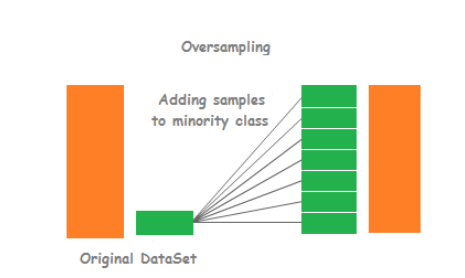
\includegraphics[width=1\textwidth]{figure4.png}}
	\centering
	\caption{Sample diagram to represent over sampling}
	\label{over sampling}
\end{figure}

\textbf{Advantages of Over Sampling:}

\begin{enumerate}
	\item When under sampling is applied, there is a loss of information because certain records are eliminated. However, when using over sampling, additional copies of the current records are created, resulting in an increase in the size of the dataset.
	\item During the process of data modelling, it becomes clear through a comparative analysis that over sampling tends to yield more favourable outcomes compared to under sampling.
\end{enumerate}



During the implementation process, the imblearn.over-sampling library has been very useful. The RandomOverSampler module played a crucial role in our analysis. The module plays an important role in both under-sampling and over-sampling procedures. In this specific situation, our main objective was to use the RandomOverSampler technique in order to tackle the issue of imbalance.

When we use the RandomOverSampler, we start a process where we duplicate records from the minority class in a random way. To implement this strategy, we need to create an instance of the random over-sampling module. Afterwards, this example is used to adjust the resample by utilising the x-train and y-train datasets. The outcome of this operation is an x-train and y-train that have been successfully over-sampled.

The current project focuses on categorising data into four different classes: benign, phishing, malware, and defacement. Each class has different occurrence frequencies and ratios. The "benign" class has the highest count, specifically 214,234 occurrences. The "defacement" class has a total of 47,611 occurrences, which is in contrast to the "phishing" class that has 47,037 occurrences. Additionally, the "malware" class has a total of 11,680 instances within the dataset.

add figure 5



Figure 3.3 illustrates the presence of a class imbalance, which leads to a decrease in accuracy and a bias in predictions towards specific classes. In order to tackle this matter, we implemented the Random Oversampling technique for the classes that have a lower number of instances. This methodology entails enhancing the dataset by creating supplementary samples for the minority classes, hence achieving balance in the distribution. The results of this evenly distributed dataset can be noticed in Figure 3.4.

The visual representation in Figure 3.4 illustrates the outcomes, indicating that there is now an equal distribution of cases across all classes in the dataset. The implemented solution has effectively addressed the initial disparity in class representation.

add figure 6


\newpage
\subsection{ Pre-Processing of Text:}

After the gathering of textual data, the subsequent essential stage involves the pre-processing of the data. The relevance of this stage is greatly focused due to its essential function in influencing the interpretation of words and characters within the data in subsequent phases\cite{Srividhya}. The utilisation of text pre-processing techniques facilitates the consolidation of diverse word forms into a single, distinct form \cite{Srividhya}. The domain of text pre-processing comprises a range of approaches, such as cleansing, tokenization, removal of stop words, lemmatization, and stemming. Within the scope of this research, we applied specialised approaches such as tokenization, stemming, and count vectorization.
\subsubsection{Tokenazation:}


Tokenization refers to the procedure of dividing large quantities of text into smaller chunks. In the course of this particular technique, the uninterrupted stream of language can be divided into discrete entities known as tokens, which include words, symbols, and phrases\cite{hickman2022}. It is imperative to acknowledge that individual characters or complete phrases are not regarded as separate entities within this procedure. The process of tokenization is limited to the manipulation of words, as they possess the capacity to communicate semantic information. A designated character, commonly known as a delimiter, is utilised for the purpose of distinguishing separate words. Occasionally, even a mere empty space can function as a delimiter. Tokenization is utilised in several domains, including but not limited to chatbot development, text categorization, and sentiment analysis. In order to improve the cleanliness of the dataset, researchers utilise a technology called regular expression (regexp). The utilisation of regular expressions, especially when dealing with extensive datasets, is strongly advised. In the context of this project, regular expressions (regexp) were employed to divide URLs into tokens or words, using the specified regexp pattern.
add figure 7


\subsubsection{Removal Of Stop Words:}
Stop words are commonly encountered words that have little or no meaningful contribution to the overall importance of a dataset. The contributions made by these elements to the offered dataset are minimal and lack substantial informative value. The dataset inherently has fundamental components that function as the fundamental units for forming phrases\cite{Srividhya}. As a result, the possibility of eliminating stop words becomes feasible. However, the necessity of removing stop words for this specific project has not been determined. Stop words are a category of words that often consist of conjunctions and prepositions. These words are considered irrelevant within a given dataset and hence do not have any meaningful value.




The utilisation of stemming has been recognised as a remarkably efficient and helpful method in the pre-processing stage. This methodology involves reducing terms within the dataset to their underlying morphological bases. By transforming words into their root forms, one can prevent any undesirable interruptions or alterations. Nevertheless, there are circumstances in which this methodology introduces significant interference. There are some words that ought to be excluded from the process of root reduction due to the fact that they maintain substantial significance in their original forms. According to\cite{hickman2022}, the simplification of words to their base forms results in the introduction of a considerable degree of superfluous intricacy, thereby reducing their overall efficiency and efficacy.

Although the efficacy of stemming is compromised by the introduction of noise caused by some words, it remains popular because to its user-friendly characteristics. Despite its inherent limitations, stemming is still widely used due to its user-friendly nature.
add figure 8




\section{Model Performances:}
\subsection{Support Vector Machine:}


The Support Vector Machine (SVM) was widely embraced as a machine learning classifier, but its prominence diminished with the emergence of neural networks and deep learning techniques. The fundamental principle underlying Support Vector Machines (SVMs) is centred on the concept of maximum margin categorization. The primary objective of this strategy is to optimise the separation margin between the two classes involved in the classification process. It is worth mentioning that Support Vector Machines (SVM) are essentially designed to do binary classification. Therefore, in order to utilise SVM for multi-class classification, more sophisticated approaches such as one vs. rest or one vs. one techniques need to be employed \cite{mahesh2020machine}.
\begin{figure}[htb]
\centerline{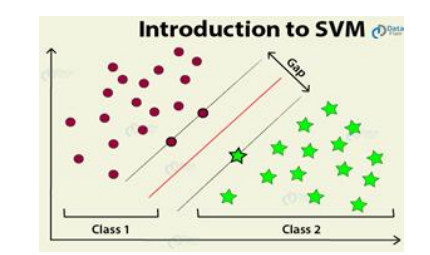
\includegraphics[width=1\textwidth]{SVMex.png}}
\caption{Support Vector Machine \cite{mahesh2020machine}}
\label{FigureSVM}
\end{figure}


As depicted in \ref{FigureSVM}, the Support Vector Machine functions as a classifier with greatest margin. The main goal is to choose the most suitable hyperplane that maximises the separation between the classes. However, in order to achieve non-linear decision boundaries, a viable strategy entails the utilisation of a kernel. The kernel in question can be understood as a hyperplane situated within a nonlinear space of higher dimensions. The efficacy of support vector machines (SVMs) stems from their utilisation of nonlinear kernel techniques, although at the expense of increased training durations.

The mathematical basis of Support Vector Machines (SVMs) is grounded in ideas of restricted optimisation. The focus of this approach is to expand the margin of the hyperplane in accordance with certain conditions: all data points belonging to one class must be situated on one side of the hyperplane, while those belonging to the other class should be located on the opposite side. The optimisation procedure described in this context is in accordance with the Karush Kuhn Tucker (KKT) conditions, which provide a comprehensive mathematical foundation for comprehending the optimisation of Support Vector Machines (SVMs).\cite{Thorsten} As a result, it is sufficient to maintain only the support vectors, which are the points located on the hyperplane, in order to completely specify the SVM classifier.

The soft margin support vector machine (SVM) is a frequently encountered variation that incorporates increased adaptability to account for possible misclassifications. The hyperparameter referred to as 'C' in Support Vector Machines (SVM) governs the level of flexibility in the margin. One notable observation is that when the value of 'C' is set to 0, the Support Vector Machine (SVM) is converted into a hard margin classifier.
\begin{figure}[htb]
\centerline{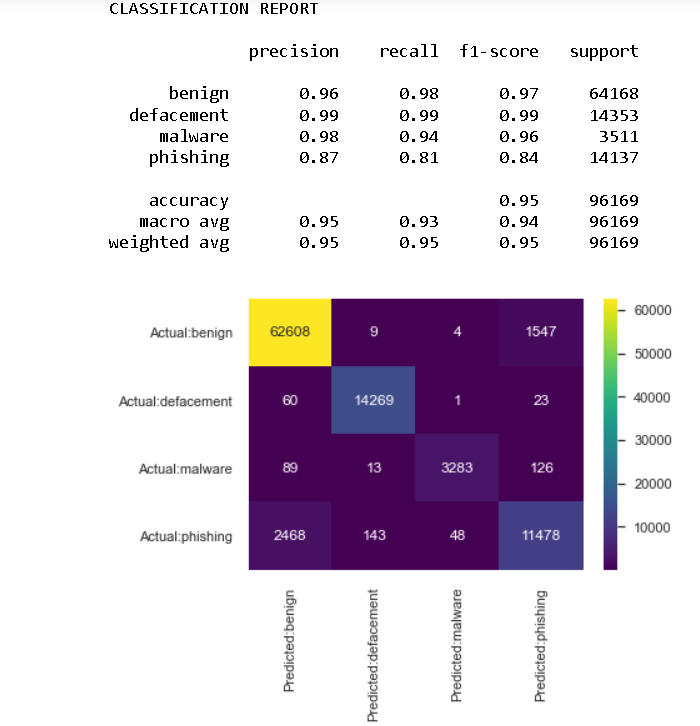
\includegraphics[width=1\textwidth]{SVMclassification.png}}
\caption{Classification and confusion matrix report of SVM}
\label{Claaification Report of SVM }
\end{figure}

In this study, it was found that the Support Vector Machine (SVM) performed extremely well. It showed a training accuracy of 99.5\% and a testing accuracy of 95.2\%. The precision for the benign class was 96\%, which is quite impressive. Similarly, the recall for the benign class was commendable at 98\%. However, it is important to mention that the execution time of the SVM was significantly long.  Figure\ref{Claaification Report of SVM } displays the comprehensive classification report and the related confusion matrix.

\subsection{Logistic Regression:}



Logistic regression is a type of classifier that is used to solve classification problems. It is an extension of linear regression, which is a method used for predicting continuous values. However, logistic regression focuses on predicting discrete outcomes by assigning probabilities to different classes. Instead of making direct predictions of numerical values, this method uses the sigmoid function to convert the output values into a range that is limited between 0 and 1.
\begin{figure}[htb]
\centerline{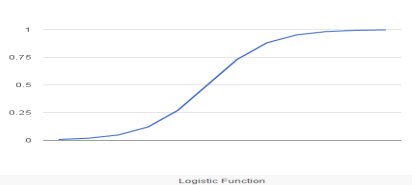
\includegraphics[width=1\textwidth]{Logisticfunction.png}}
\caption{Logistic Function \cite{Naresh_Gupta_Giri_2020}}
\label{logistic function }
\end{figure}

 \begin{equation*}{\text{ Logistic Function \cite{Chiramdasu}}}:  \frac{1}{{\left({1 + {e^{ - x}}}\right)}},\tag{1}\end{equation*} 
 \hfill \goodbreak
           where e is constant, and x is input

The sigmoid function is used to compress the output values between 0 and 1, which helps in making classification decisions. When the value of g(x), which is the output of the sigmoid function, becomes greater than 0.5, the instance is classified into a particular category, such as(malicious). On the other hand, when the value of g(x) is less than 0.5, the classifier categorises the instance as (non-malicious)\cite{Naresh_Gupta_Giri_2020}.

The loss function measures the difference between the actual category of a training example and the category that the model predicts. Linear regression often uses the squared loss, but logistic regression uses the binary cross-entropy loss for binary classification and the categorical cross-entropy loss for tasks with multiple classes.

The mathematical representation of the binary cross-entropy loss is given by the formula:
           $$-(ylog(p) + (1 - y)log(1 - p))$$
. In this formula, 'y' represents the true class label, and 'p' represents the predicted class label for a specific test instance.

The main goal of logistic regression is to minimise the cumulative cross-entropy loss for the entire training dataset. To achieve this objective, we need to use optimisation techniques to make the learning process more efficient. This will help us improve the model's ability to make accurate predictions.





\begin{figure}[hb]
\centering
\centerline{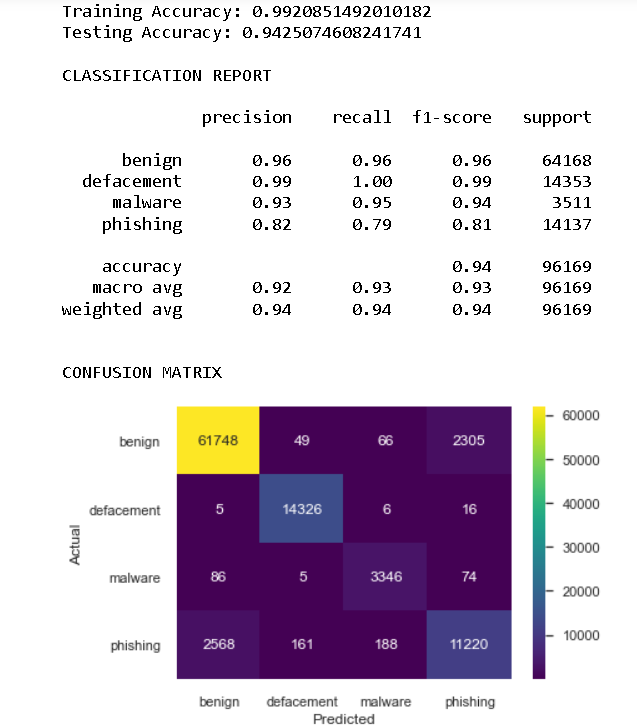
\includegraphics[width=1\textwidth]{LogisticRegressionreport.png}}
\caption{Classification and confusion matrix report of Logistic Regression}
\label{Claaification Report of LR }
\end{figure}







In this study, we utilised logistic regression to obtain significant results. During the training phase, the accuracy rate achieved was quite impressive at 99.2\%. Similarly, when the model was tested, it showed a beneficial accuracy of 94.2\%. When we examine the classification report as shown in figure\ref{Claaification Report of LR }, we can observe the precision scores for different categories such as benign, defacement, and malware. This analysis helps us understand how effective these precision scores are in accurately classifying the data . However, it is important to mention that the precision score for phishing does not meet the expected standards. When examining the confusion matrix, we can see that there were 64,168 actual benign values. Out of these, 2305 URLs were incorrectly classified as phishing. This raises concerns about potential suspicious activities.

\subsection{Random Forest:}



Random Forest classifiers are built upon decision trees as their fundamental basis. The reason why they are so popular is because they are really good at accurately classifying things, even though they require a lot of time to train. The main idea behind Random Forests is called bagging, which is a technique used in machine learning. Bagging involves using multiple models together to make predictions. Instead of only using the results of one model, this approach proposes training multiple different models and then combining their predictions. Techniques such as majority voting or averaging can be used to achieve a mix of results from diverse models. The strategies that have been shown have improved the ability to make predictions.

Random Forests can be described as a collection of multiple decision trees that come together to form a 'forest.' The decision trees in this forest may have different depths, which is determined by pruning. In a typical Random Forest setup, it is common to use a collection of 100 or 200 decision trees to achieve the desired outcomes.

\begin{figure}[h]
\centering
\centerline{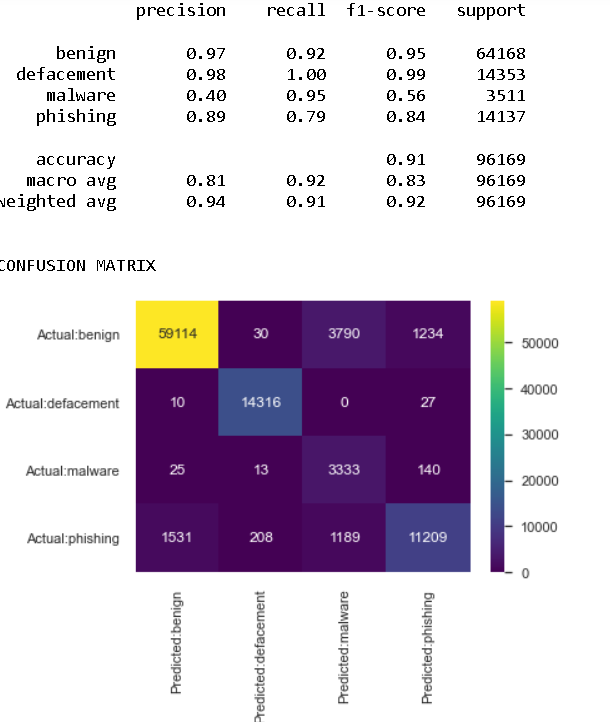
\includegraphics[width=1\textwidth]{RFclassification.png}}
\caption{Classification and confusion matrix report of Random Forest}
\label{Claaification Report of RF }
\end{figure}



In this project, we found that the Random Forest technique performed really well. It had high accuracy rates during both the training phase (99.9\%) and the testing phase (91.4\%). When examining the benign class, we calculated precision and recall scores of 92\% and 97\%, respectively.Foe more understanding we can refer to the\ref{Claaification Report of RF } the classification report and confusion matrix shown in the accompanying figure.

\subsection{Decision Tree:}


Decision trees (DT) are a method that is not parametric commonly used in supervised learning for the purposes of classification and regression. What exactly distinguishes them is their capacity to function efficiently with minimal pretreatment of data \cite{YANG201361}, in contrast to certain alternative classification methods that need procedures such as data normalisation, generation of dummy variables, or handling missing values. It is important to note that data transformers (DTs) do not possess an intrinsic capability to manage missing values. From a visual perspective, a decision tree (DT) can be metaphorically compared to a hierarchical structure resembling a tree, where the qualities are represented as nodes. A compelling recurrent pattern emerges during the process of classification.

\begin{figure}[htb]
\centering
\centerline{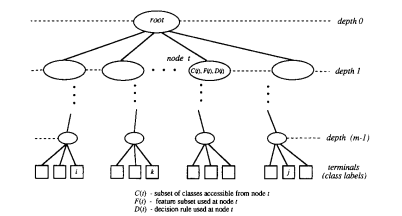
\includegraphics[width=1\textwidth]{DTexample.png}}
\caption{Example of Decision Tree Classifier}
\label{example DT }
\end{figure}

In essence, decision trees (DTs) consist of a collection of nodes originating from a single root node as shown in the above figure\ref{example DT }, with each of these nodes subsequently branching out into various directions. One intriguing characteristic of this particular structure is that the root node does not have any incoming edges, yet all succeeding nodes, also known as leaves \cite{YANG201361}, have precisely one incoming edge. As the classification process progresses, it is possible for these leaves to divide into sub-nodes under the guidance of the input training data. It is important to acknowledge that within every leaf node, there exists a probability vector that functions as an indicator of the likelihood associated with particular values of the target property.

The accuracies obtained for both the training and testing phases are 85\% each. The precision and recall scores for the "benign" category are significant, with values of 86\% and 95\% respectively. The comprehensive classification report and the confusion matrix for the decision trees model are displayed in Figure \ref{Classification and confusion matrix report of DT } for reference.

\begin{figure}[htb]
\centering
\centerline{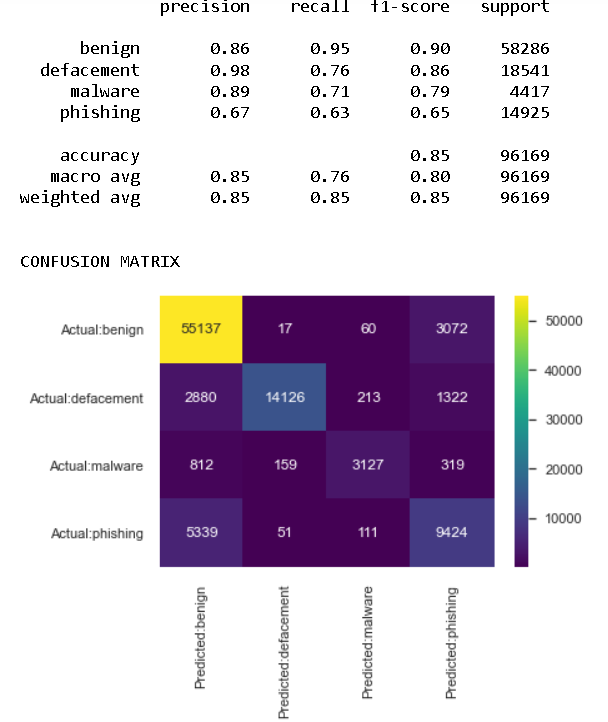
\includegraphics[width=1\textwidth]{DTclassification.png}}
\caption{Classification and confusion matrix report of Decision Tree}
\label{Classification and confusion matrix report of DT }
\end{figure}

\newpage
\section{Hyperparameter Tuning}



Parameters are crucial components of machine learning models, since they are responsible for their initialization and ongoing adjustment during the learning process. whereas,\cite{YANG201361} hyperparameters play a crucial role in determining the specific parameters that contribute to maximising the accuracy of the model. The hyperparameters can be manually specified or initialised by methods such as grid search cross-validation or randomised search cross-validation.

It is crucial to acknowledge that the determination of hyperparameters cannot be immediately inferred from the training data alone. However, it is imperative that these factors are determined prior to initiating the training process of a machine learning model. The hyperparameters play a crucial role in guiding the model to select the method that minimises the loss function. Consequently, the efficacy of machine learning algorithms can be significantly improved by engaging in the practise of fine-tuning, which entails the systematic examination of various parameter combinations.

Within the realm of machine learning algorithms, a wide range of parameters can be observed. The quantity and characteristics of these factors can vary considerably across different algorithms. The process of fine-tuning algorithms by modifying various parameters ultimately leads to the determination of the most optimal parameter configurations for any specific algorithm\cite{YANG201361}.


\newpage
\section{Cross Validation}



In a machine learning data science project, it is crucial to recognise the significance of each phase, starting from data collection to model deployment. The first step is to divide the dataset into two sets: the training set and the testing set. For this specific project, the data was divided into a training dataset of 70\% and a testing dataset of 30\%. The training dataset, which makes up 70\% of the data, is used to train the model. However, the remaining 30\% of the data, which is known as the test data, is used to evaluate the accuracy of the model.

The process of splitting data into training and testing subsets includes a random selection procedure. The randomness in this situation brings about uncertainty, which could result in cases where specific data in the testing set may not exist in the training set. As a result, this discrepancy can have a detrimental effect on the accuracy of the model. In order to tackle this concern, we can turn to the concept of K-fold cross-validation, which provides a more reliable way to assess prediction error.

In terms of computational efficiency,\cite{wong2019reliable} K-fold cross-validation is commonly preferred over leave-one-out cross-validation. The random state parameter used in the train-test split can be set to any numerical value. The selection of data points is determined by the choice of this random state number. When we change the random state number, it causes different sets of data points to be selected. This, in turn, leads to variations in the accuracy outcomes.

The K-fold cross-validation technique is introduced to reduce variability and improve accuracy assessment. Having a sufficient amount of training data is extremely important when it comes to constructing a dependable model. In K-fold cross-validation\cite{yadav2016analysis}, the dataset is split into training and testing subsets using a specific integer value called 'k.' Every value of 'k' represents a different experiment. In this example, we have a dataset with 10,000 records. We will be conducting five experiments, with 'k' set to 5.

For the first experiment, we use the first 2,000 records for training and keep the remaining 8,000 records for testing. In the following experiments, the model is trained using the next 2,000 records and then evaluated using the same set of 8,000 records. The purpose of this rotation is to ensure that the data points used for training in one experiment are used as the testing data in subsequent experiments. The iterative process will continue until all five experiments have been completed. The experiments produce five different accuracy values, and the final accuracy is determined by finding the average of these values.



\newpage
\section{Metrics for classifier evaluation:}
\subsection{Accuracy:}


The idea of accuracy is about determining the ratio of correct predictions to all the predictions made. Accuracy faces a difficulty when tackling classification tasks that have a noticeable imbalance among various classes. The problem becomes evident when one specific class has a significantly larger representation in the dataset. In situations like these, if we consistently predict the dominant class, it may lead to a high accuracy score. Regrettably, this demonstration does not effectively highlight the model's ability to accurately predict the minority class, which typically exhibits lower accuracy\cite{javaid2016deep}\cite{yacouby-axman-2020-probabilistic}.



Predictions are divided into four separate categories, namely True Positive (TP), False Positive (FP), True Negative (TN), and False Negative (FN). When a positive test result matches a positive prediction correctly, we call it a True Positive (TP). On the other hand, when a positive test result goes against a correct negative prediction, it is called a False Positive (FP). In the same way, when a negative test result aligns with an accurate negative prediction, it is referred to as a True Negative (TN). On the other hand, if a negative test result goes against a correct positive prediction, it is considered a False Negative (FN).

\subsection{Precision:}



Precision, also known as Positive Prediction Value, is a measure that evaluates the accuracy of positive predictions. The quantification of it is primarily determined by calculating the ratio of True Positives (TP) to the total number of instances that were predicted as positive. The main focus of this metric is to reduce errors, especially when it comes to accurately predicting positive labels\cite{javaid2016deep}\cite{yacouby-axman-2020-probabilistic}. The formula for precision can be expressed in the following manner:

\[
\text{Precision} = \frac{\text{True Positives}}{\text{True Positives} + \text{False Positives}}
\]





\subsection{Recall:}



Recall is the term used to describe the process by which the model derives information based on the genuine facts that are available. The term used to refer to the True Positive Rate (TPR) or sensitivity is also known as such. The reason for using this terminology is because the projected values are obtained as positive values, which aligns with the existing True Positives (TP) in the given scenario. One challenge that arises with recall is its tendency to classify all instances as positive cases, which can have a negative impact on the overall performance scores of the model. TPR, also known as True Positive Rate, is a measure that compares the number of True Positives to the total of True Positives and False Negatives\cite{javaid2016deep}\cite{yacouby-axman-2020-probabilistic}. The formula for recall is given as follows:

$$\text{Recall} = \frac{\text{True Positives}}{\text{True Positives} + \text{False Negatives}}$$


\subsection{F1 Score:}


The F1 score is considered the most preferred metric for demonstrating the performance of a model. The way it works is by comparing various systems and evaluating how effectively the model performs in comparison to them. The score is typically calculated based on the precision and recall values of the model. In situations where there are multi-class systems, the F1 score might not give completely satisfactory results because there is no true negative reference. The lack of true negatives is also applicable when measuring recall and precision\cite{yacouby-axman-2020-probabilistic}.

The F1 score is a metric that combines precision and recall in a balanced way. The metric scores obtained from evaluating classification models usually range from 0 to 1. A score of 1 suggests that the model's performance is commendable.

 $$ F1 = 2 \cdot \frac{precision \cdot recall}{precision + recall} $$

 \subsection{Confusion Matrix:}
 

The utilisation of a confusion matrix arises when there is a need to visually depict the degree of concordance between our predictive outcomes and the true categories. A representation of this matrix can be observed in Figure\ref{example CM }\cite{ARAVINDA20221}. Various assessment metrics can be derived from this matrix, encompassing recall, precision, and the F1 score, among others.

\begin{figure}[h]
\centering
\centerline{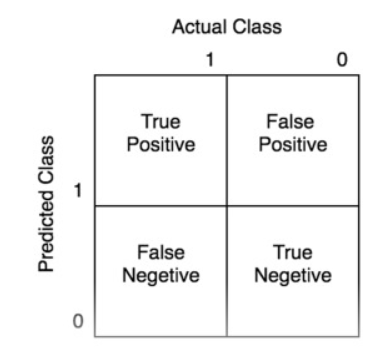
\includegraphics[width=1\textwidth]{confusionexample.png}}
\caption{Example of Confusion Matrix adopted from \cite{ARAVINDA20221}}
\label{example CM }
\end{figure}







